\chapter{Background Knowledge and Related Work}
%OR: \chapter{Tools and Methods}
\label{cha:background-theory}

\begin{comment}
The background theory depth and breadth depend on the depth needed to understand your project
in the different disciplines that your project crosses.
It is not a place to just write about everything you know that is vaguely connected to your project.
The theory is here to help the readers that do not know the theoretical basis of your work so that they
can gain sufficient understanding to understand your contributions --- and also for yourself to show that
you have understood the underlying theory and are aware of the methods used in the field.
In particular, the theory section provides
an opportunity to introduce terminology that can later be used without disturbing the text with a definition.
In some cases it will be more appropriate to have a separate section for different theories (or even separate chapters).
However, be careful so that you do not end up with too short sections.
Subsections may also be used to separate different background theories.

Be aware that ``background'' is a general term that refers to everything done by somebody else,
in contrast to the ``foreground'', which is your own work.
Hence there can (and will) be several background chapters, with the background theory being one of them
--- or several of them, since it thus is quite possible to split the background theory over more than one chapter,
e.g., by having a chapter introducing the theory directly needed for the research field in question and another
chapter discussing the machine learning theory, algorithms, tools, and evaluation methods commonly used in the field.
The related work chapter is thus also part of the background, while a chapter about data might be background
(if you only use somebody else datasets), but can also be part of the foreground (if you collect and/or annotate data
yourself, or if you process or clean the data in ways that can make it part of your own contribution).

It is ok to reuse material from other texts that you have written (e.g., the specialisation project), but if you do so, that must be clearly stated in the text, together with a description of how much of the text is new, old or rewritten/edited.
Such a statement about recycling of material in the Background Theory chapter can thus come here in the chapter introduction.

\section{Writing References in the Text}
\label{sec:writing_references}

When introducing techniques or results, always reference the source.
Be careful to reference the original contributor of a technique and not just someone who happens to use the technique.%
\footnote{But always make sure that you have read the work you are citing --- if not, cite someone who has!}
For results relevant to your work,
you would want to look particularly at newer results so that you have referenced the most up-to-date work in your area.
A common rule of thumb is to at least reference the first paper introducing the issue and the paper containing the latest / state-of-the-art
results. Additional papers making substantial contributions should also be referenced, as well as of course the ones you find most interesting.
Remember to use the right verb form depending on the number of authors.

If you do not have the source handy when writing, mark in the text that a reference is needed and add it later. \todo{add reference}
Web pages are not reliable sources --- they might be there one day and removed the next; and thus should be avoided, if possible.
A verbal discussion is not a source and should normally not be referenced
(though you can reference ``personal communication'', if there are no other options).
The bulk of citations in the report will appear in Chapter~\ref{cha:related_work}.
However, you will often need to introduce some terminology and key citations already in this chapter.

You can cite a paper in the following manner (and several other versions,
see the \verb!natbib! package documentation):

\begin{enumerate}[(i)]
    \item When referring to authors, using their names in the text:\\
          \citet{Authorson;Bobsen:10} stated something rather nice.
          (using \verb!\citet!)
    \item To cite indirectly: \\
          Papers should be written nicely \citep{Authorson;Bobsen:10}
          (using \verb!\citep!)
          {\em or\/}\\
          In \citet{Authorson;Bobsen:10}, a less detailed template was presented.
    \item To just cite the authors: \\
          \citeauthor{Authorson;Bobsen:10} wrote a nice paper
          (using \verb!\citeauthor!).
    \item Or just the year: \\ \citeyear{Authorson;Bobsen:10}
          (using \verb!\citeyear!).
    \item You can even cite specific pages or chapters: \citet[p. 3]{Authorson;Bobsen:10}
          (using \verb!\citet[...]{...}!).
\end{enumerate}

You should obviously always cite your supervisor's work \citep{BenyonEA:13},
even if it is completely irrelevant \citep{Das;Gamback:13a} or very old \citep{AlshawiEA:91b}.
Digging up an even older book can also appear impressive \citep{Diderichsen:57}.
(Or? ;-)

\section{The Reference List}
\label{sec:reference_list}

In general, make sure that the references that appear in your reference list can be easily located and identified by the reader.
So include not only authors and title, but year and place of publication, the full names of conferences and workshops,
page numbers in proceedings and collections, etc.
Hyperlinks or \acrfull{acr:doi} numbers are also nice to include.
Just as in the text itself, it is important to be consistent in the reference list, so include the same type of information for all references and write it in the same way.

Check out the reference list at the end of this document for examples of how to write references in \BibTeX.
Note a particular quirk: Many \BibTeX\ styles convert uppercase letters to lowercase, unless specifically told not to.
You might thus need to ``protect'' characters that should not be converted, e.g., by writing \texttt{\{T\}witter} as in the \citet{FountaEA:18} reference.

Also, keep in mind that `et' is a word in its own right (`and'), so there is no period after it (even though there is a period after `al.', which is short for `alia', meaning `others').
Of course, when including such a reference in the text, the authors should be referred to in plural form.
So \citet{BenyonEA:13} state that life is good (not ``states'').

Many sites, such as journals and \url{dblp.org} provide the matching \BibTeX\ entry for a reference.
However, you might still need to edit the entry in order to be consistent with the rest of your references.
If you find references from sites such as \url{scholar.google.com} or \url{arXiv.org}, keep in mind that they often not are complete,
so that you might need to add information to the entry (and probably edit it as well).

Some other good sites to find state-of-the-art work:
\begin{itemize}
    \item \url{paperswithcode.com}
    \item \url{nlpprogress.com}

\end{itemize}

\textit{Lorem ipsum dolor sit amet, consectetur adipiscing elit, sed do eiusmod tempor incididunt ut labore et dolore magna aliqua. Ut enim ad minim veniam, quis nostrud exercitation ullamco laboris nisi ut aliquip ex ea commodo consequat. Duis aute irure dolor in reprehenderit in voluptate velit esse cillum dolore eu fugiat nulla pariatur. Excepteur sint occaecat cupidatat non proident, sunt in culpa qui officia deserunt mollit anim id est laborum.}

\begin{figure}[t!]
    \centering
    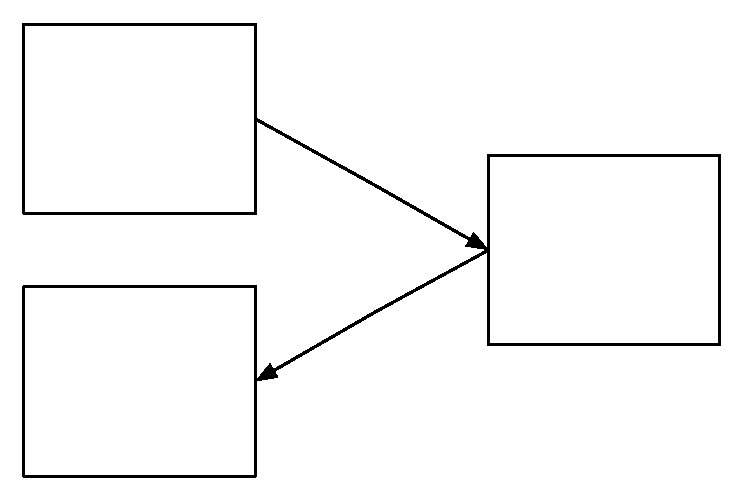
\includegraphics[width=0.5\columnwidth]{figs/figure1.pdf}
    \caption[Boxes and arrows are nice]{Boxes and arrows are nice (adapted from \citealp{Authorson;Bobsen:10}, reprinted with permission)}
    \label{fig:BoxesAndArrowsAreNice}
\end{figure}

\section{Introducing Figures}

\LaTeX is a bit tricky when it comes to the placement of ``flooting bodies'' such as figures and tables. It is often a good idea to let their code appear right before the header of the (sub)section in which they appear.
Note that you should anyhow always use an option for the placement (e.g., \verb|[t!]| to place it at the top of a page).

Remember that if you reproduce someone else's figures you must credit the original author --- such as
Figure~\ref{fig:BoxesAndArrowsAreNice} (adapted from \citealp{Authorson;Bobsen:10}),
as well as state that you have permission to reprint it (e.g., if it is published under a Creative Commons License,
or if you have gained explicit permission from the author).

Do not just put the figure in and leave it to the reader to try to understand what the figure is.
The figure should be included to convey a message and you need to help the reader to understand the message
intended by explaining the figure in the text.
Hence \textbf{all} figures and tables should always be referenced in the text, using the \verb!\ref! command.
It is good practice to always combine it with a non-breakable space (\verb!~!) so that there will be no newline between the term referring to it and the reference, that is, using \verb!Figure~\ref{fig:BoxesAndArrowsAreNice}!.

If a figure appears far from the text explaining it,
it is a good idea to add its page number (using the \verb!\pageref! command), so that you can refer to Figure~\ref{fig:BoxesAndArrowsAreNice} (on Page~\pageref{fig:BoxesAndArrowsAreNice}).

Also, note that you can have a longer version of the figure (and table) caption attached to the actual figure,
while using the optional first argument to \verb!\caption! to include a shorter version in the list of figures (lof) or list of tables:
\begin{quote}
    \begin{verbatim}
\caption[Shorter lof text]{Longer text appearing under the figure}
\end{verbatim}
\end{quote}

It is good practice to add a note about a missing figure in the text,
such as the completely amazing stuff that will appear in Figure~\ref{fig:AmazingFigure}.

\begin{figure}[t!]
    \centering
    \missingfigure{Here we will add an amazing figure explaining it all}
    \caption{A missing figure}
    \label{fig:AmazingFigure}
\end{figure}

In general it is good to add notes about things that you plan on writing later.
The \verb!todonotes! package is great for that kind of book-keeping, letting you write both shorter comments in the margin\todo{l8r dude} and longer comments inside the text, using the option \verb![inline]!.
\todo[inline]{There are always some more stuff that you will need to add at some later point.
    Be sure to at least make a note about it somewhere.}

\textit{Sed ut perspiciatis unde omnis iste natus error sit voluptatem accusantium doloremque laudantium, totam rem aperiam, eaque ipsa quae ab illo inventore veritatis et quasi architecto beatae vitae dicta sunt explicabo. Nemo enim ipsam voluptatem quia voluptas sit aspernatur aut odit aut fugit, sed quia consequuntur magni dolores eos qui ratione voluptatem sequi nesciunt. Neque porro quisquam est, qui dolorem ipsum quia dolor sit amet, consectetur, adipisci velit, sed quia non numquam eius modi tempora incidunt ut.}

\section{Introducing Tables in the Report}

\newcommand\emc{-~~~~}
\begin{table}[t!]
    \centering
    \caption[Example table]{Example table (F$_1$-scores); this table uses the optional shorter caption that will appear in the list of tables, so this long explanatory text will not appear in the list of tables and is only here in order to explain that to the reader.}
    \begin{tabular}{c|c|rrrrrr}
        \tabletop
        Langs                  & Source                                           & \multicolumn{1}{c}{Lang1} & \multicolumn{1}{c}{Lang2} & \multicolumn{1}{c}{Univ} & \multicolumn{1}{c}{NE} & \multicolumn{1}{c}{Mixed} & \multicolumn{1}{c}{Undef}
        \\ \tablemid
        \multirow{5}{*}{EN-HI} & FB+TW                                            & 54.22                     & 22.00                     & 19.70                    & 4.00                   & 0.05                      & 0.03                      \\
                               & FB                                               & 75.61                     & 4.17                      & 18.00                    & 2.19                   & 0.02                      & 0.01                      \\
                               & TW                                               & 22.24                     & 48.48                     & 22.42                    & 6.71                   & 0.08                      & 0.07                      \\
                               & Vyas                                             & 54.67                     & 45.27                     & 0.06                     & \emc                   & \emc                      & \emc                      \\
                               & FIRE                                             & 45.57                     & 39.87                     & 14.52                    & \emc                   & 0.04                      & \emc                      \\ \tablemid
        \multirow{2}{*}{EN-BN} & TW                                               & 55.00                     & 23.60                     & 19.04                    & 2.36                   & \emc                      & \emc                      \\
                               & FIRE                                             & 32.47                     & 67.53                     & \emc                     & \emc                   & \emc                      & \emc                      \\ \tablemid
        EN-GU                  & FIRE                                             & 5.01                      & \textbf{94.99}            & \emc                     & \emc                   & \emc                      & \emc                      \\
        \tablemid
        DU-TR                  & Nguyen                                           & 41.50                     & 36.98                     & 21.52                    & \emc                   & \emc                      & \emc                      \\ \tablemid

        EN-ES                  & \multirow{4}{*}{\rotatebox[origin=c]{90}{EMNLP}}
                               & 54.79                                            & 23.50                     & 19.35                     & 2.08                     & 0.04                   & 0.24                                                  \\
        EN-ZH                  &                                                  & 69.50                     & 13.95                     & 5.88                     & 10.60                  & 0.07                      & \emc                      \\
        EN-NE                  &                                                  & 31.14                     & 41.56                     & 24.41                    & 2.73                   & 0.08                      & 0.08                      \\
        AR-AR                  &                                                  & 66.32                     & 13.65                     & 7.29                     & 11.83                  & 0.01                      & 0.90                      \\ \tablebot
    \end{tabular}
    \label{tab:ExampleTable}
\end{table}

As you can see from Table~\ref{tab:ExampleTable}, tables are nice.
However, again, you need to discuss the contents of the table in the text.
You do not need to describe every entry, but draw the reader's attention to what is important in the table,
e.g., that 94.99 is an amazing F$_1$-score (and that probably something fishy happened there).
Use boldface, boxes, colours, arrows, etc. to mark the important parts of the table.

As can be seen in the example, elements in a table can sometimes benefit from being rotated (such as EMNLP in the `Source' column) or cover more than one row (EMNLP, as well as EN-HI and EN-BN in the `Langs' column) --- or more than one column, for that matter.

\textit{Donec non turpis nec neque egestas faucibus nec id neque. Etiam consectetur, odio vitae gravida tempus, diam velit sagittis turpis, a molestie ligula tellus at nunc. Proin dolor neque, dapibus a pellentesque a, commodo a nibh.}
\end{comment}

\begin{itshape}
    NB! Parts of the \nameref{cha:background-theory} chapter is reused material from the specialization project \citep{holmLLMsDeathGIS2023} that preceded this master's thesis. Below are the sections in question and the extent to which, and how, the materials are reused:

    \begin{itemize}
        \item \Autosubsectionref{subsec:attention-and-the-transformer-architecture}: Reused, with minor adjustments.
        \item \Autosubsectionref{subsec:sota-decoder-only-llms}: \acrshort{acr:gpt} part reused without modifications.
        \item \Autosubsectionref{subsec:llm-gis}: Reused, with minor adjustments.
    \end{itemize}
\end{itshape}

\vspace{12pt}

\noindent \Autochapterref{cha:background-theory} will lay a theoretical basis for the work done in this master thesis, providing the user with the necessary knowledge to understand the contributions of the work. It will also provide an overview of previous research that shares objectives similar to those of this thesis. \Autosectionref{sec:llms} will focus on \gls{acr:llm}. First, \autoref{subsec:core-concepts} will introduce the terms \enquote{tokens} and \enquote{context window}, which are terms used frequently throughout this thesis. Thereafter, \autoref{subsec:attention-and-the-transformer-architecture} will present the component that most modern \glspl{acr:llm} are based upon --- namely the Transformer --- and the attention mechanism that drives it. Continuing, \autoref{subsec:sota-decoder-only-llms} section will present some of the leading \acrshortpl{acr:llm} as of \today, both proprietary and open-source ones. \Autosubsectionref{subsec:prompt-engineering} will present the concept of \textit{prompt engineering}, which is a structured way of composing an input to the \acrshort{acr:llm}, before \autoref{subsec:function-calling} concludes \autoref{sec:llms} by presenting \textit{function calling}, a way of allowing \acrshortpl{acr:llm} to use external tools. \Autosectionref{sec:langchain} will give a brief intro to LangChain, a Python/JavaScript library that is used extensively throughout the code base of GeoGPT. \Autosectionref{sec:geo-dbs-and-data-catalogues} will introduce the reader to PostGIS, \acrshort{acr:ogc} \acrshort{acr:api} Features, and \acrshort{acr:stac} \acrshortpl{acr:api}. The first two are geospatial technologies that are used within GeoGPT. \Autosectionref{sec:related-work} will present that relates in some way to this thesis. \Autosubsectionref{subsec:llm-gis} present work where \acrshort{acr:llm} are applied for geospatial purposes, while \autoref{subsec:agent-patterns} describes different agent patterns that can be applied to \acrshort{acr:llm}-based agents to improve their performance.


\section[Large Language Models]{\acrlongpl{acr:llm}}
\label{sec:llms}

This section will lay the theoretical groundwork required to gain an overview of the inner workings of \glspl{acr:llm}. \glspl{acr:llm} are a type of neural networks that excel at language processing. They can be developed for different \gls{acr:nlp} tasks, such a text classification, masked language modelling, and text generation. While they all have their use cases, only text generation will be relevant for this thesis. Generative \glspl{acr:llm} are designed to generate some output sequence based upon some input sequence, and are the types of models behind technologies like OpenAI's \textit{ChatGPT} \citep{openaiIntroducingChatGPT2022}. This input sequence is also known as the \enquote{context window}, and all sequences are made up from \enquote{tokens}, as \autoref{subsec:core-concepts} will explain.


\subsection{Tokens and the Context Window}
\label{subsec:core-concepts}

While humans understand sentences as sequences of words, \acrshortpl{acr:llm} perceive them as sequences of \textbf{tokens}. An \acrshort{acr:llm} possesses a fixed set of unique tokens in its vocabulary, from which it constructs words and sentences. Tokens can be entire words, short character sequences, or single characters. \autoref{fig:tokenization-example-sentence} illustrates how the OpenAI's \acrshort{acr:gpt}-3.5 and \acrshort{acr:gpt}-4 models \textit{tokenize} an English sentence. Notice how some words are deconstructed into more than one token. For example, the word \enquote{revolutionizing} is split into its root, \enquote{revolution}, and its suffix, \enquote{izing}. \autoref{fig:tokenization-revolution} shows how this process applies to other suffixes as well. This way, the model only has to learn the meaning of \enquote{revolution}, and can append different suffixes to modify its function within a sentence, as opposed to learning an entirely new token for each version of the word.

\begin{figure}[htp]
    \centering
    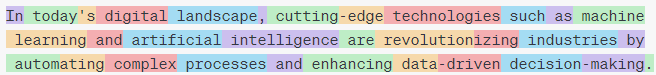
\includegraphics[width=\textwidth]{tokens_illustration.png}
    \caption{Tokenization example for an English sentence}
    \label{fig:tokenization-example-sentence}
\end{figure}

\begin{figure}[htp]
    \centering
    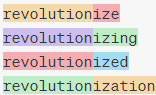
\includegraphics[width=0.25\textwidth]{revolution_tokens.png}
    \caption{Tokenization of the word \enquote{revolution} with different suffixes}
    \label{fig:tokenization-revolution}
\end{figure}

The \textbf{context window} of an \acrshort{acr:llm} is the range of tokens that an \acrshort{acr:llm} is able to process. When an \acrshort{acr:llm} generates text, it does so by generating a new token based on the tokens it sees in the span of the context window. A larger context window will allow an \acrshort{acr:llm} to take more and longer documents as context, and generate answers based on these. Leveraging sophisticated techniques like \gls{acr:rope} \citep{suRoFormerEnhancedTransformer2024} and \gls{acr:pose} \citep{zhuPoSEEfficientContext2024}, reserchers have able to efficiently extend the context window of open-source models like, for instance, Meta AI's \acrshort{acr:llama} models.


\subsection{Attention and the Transformer Architecture}
\label{subsec:attention-and-the-transformer-architecture}

\cite{vaswaniAttentionAllYou2017} managed to achieve new state-of-the-art results for machine translation tasks with their introduction of the Transformer architecture. The Transformer has later been proved effective for numerous downstream tasks, and for a variety of modalities. Titling their paper \citetitle{vaswaniAttentionAllYou2017}, \citeauthor{vaswaniAttentionAllYou2017} suggest that their attention-based Transformer architecture renders network architectures like \glspl{acr:rnn} redundant, due to its superior parallelization abilities and the shorter path between combinations of position input and output sequences, making it easier for the model to learn long-range dependencies \citep[6]{vaswaniAttentionAllYou2017}.

The Transformer employs self-attention, which enables the model to draw connections between arbitrary parts of a given sequence, bypassing the long-range dependency issue commonly found with \glspl{acr:rnn}. An attention function maps a query and a set of key-value pairs to an output, calculating the compatibility between a query and a corresponding key \citep[3]{vaswaniAttentionAllYou2017}. Looking at \citeauthor{vaswaniAttentionAllYou2017}'s proposed attention function \eqref{eq:attention}, we observe that it takes the dot product between the query $Q$ and the keys $K$, where $Q$ is the token that we want to compare all the keys to. Keys similar to $Q$ will get a higher score, i.e., be \textit{more attended to}. These differences in attention are further emphasized by applying the softmax function. The final matrix multiplication with the values $V$ (the initial embeddings of the input tokens) will yield a new embedding in which all individual tokens have some context from all other tokens. The attention mechanism is improved by multiplying queries, keys, and values with \textit{learned} weight matrices that are obtained through backpropagation. Self-attention is a special kind of attention in which queries, keys, and values are all the same sequence.

\begin{equation}
    \text{Attention}(Q, K, V) = \text{softmax}\left(\frac{QK^T}{\sqrt{d_k}}\right)V
    \label{eq:attention}
\end{equation}

Attention blocks can be found in three places in the Transformer architecture \citep[5]{vaswaniAttentionAllYou2017}. Below is an example using translation from Norwegian to German, showing how the attention blocks are used:

\begin{enumerate}
    \item In the encoder block, to perform self-attention on the input sequence (which is in Norwegian)
    \item In the decoder block, to perform self-attention on the output sequence (which is in German)
    \item In the decoder block, to perform cross-attention (also known as encoder-decoder attention) where each position in the decoder attends to all positions in the encoder
\end{enumerate}

The Transformer represented a breakthrough in the field of \gls{acr:nlp}, and is the fundamental building block of most modern \glspl{acr:llm}.


\subsection[State-of-the-Art Decoder-Only Models]{State-of-the-Art Decoder-Only \acrlongpl{acr:llm}}
\label{subsec:sota-decoder-only-llms}

While the work of \citeauthor{vaswaniAttentionAllYou2017} is still considered perhaps the greatest breakthrough in \gls{acr:nlp}, most moderns \acrshort{acr:llm} do not apply this exact encoder-decoder architecture. The evolution following the Transformer has favoured generative decoder-only models, focusing entirely on the generative component of the Transformer. The goal is to create models that can produce coherent and context-aware text.

\subsubsection{The GPT Family}
\label{subusubsec:gpt}

\gls{acr:gpt} is an \acrshort{acr:llm} that was introduced by OpenAI in 2018 \citep{radfordImprovingLanguageUnderstanding2018}. Specifically designed for text generation, a \acrshort{acr:gpt} is essentially a stack of Transformer \textit{decoders}. It demonstrates through its vast pre-training on unlabelled data that such unsupervised training can help a language model learn good representations, providing a significant performance boost while alleviating the dependence on supervised learning. While the original Transformer architecture as described by \cite{vaswaniAttentionAllYou2017} was intended for machine translation --- thus having encoders to learn the representation of the origin language representation of a given input sequence and decoders to learn the representation in the target language and perform cross-attention between the two --- the \acrshort{acr:gpt} is designed only to \textit{imitate} language. This is why there are no encoders to be found in the \acrshort{acr:gpt} architecture, only decoders. The model employs masked multi-head attention (running the input sequence through multiple attention heads in parallel), and is restricted to only see the last $k$ tokens --- with $k$ being the size of the context window --- and tasked to predict the next one.

Training consists of two stages: unsupervised pre-training and supervised fine-tuning. The former is used to find a good initialization point, essentially teaching the model to imitate the corpora upon which it is trained. This results in a model that will ramble on uncontrollably, simply attempting to elaborate upon the input sequence it is given, to the best of its abilities. This will naturally produce undefined behaviour, and it is therefore necessary to fine-tune the model on target tasks in a \textit{supervised} manner. \cite[4]{radfordImprovingLanguageUnderstanding2018} explain how the model can be fine-tuned directly on tasks like text classification, but also how other tasks require the conversion of structured inputs into ordered sequences, as is the case when fine-tuning for tasks like multiple choice (see \autoref{fig:multiple-choice}). This \textit{inlining} is required because the pre-trained model was trained on contiguous sequences of text. In the case of ChatGPT, \citeauthor{openaiIntroducingChatGPT2022} used \gls{acr:rlhf} \citep{christianoDeepReinforcementLearning2023} by employing a three-step strategy: first training using a supervised policy, then using trained reward models to rank alternative completions produced by ChatGPT models, before fine-tuning the model using \gls{acr:ppo} \citep{schulmanProximalPolicyOptimization2017}, which is a way of training \acrshort{acr:ai} policies. This pipeline is then performed for several iterations until the model produces the desired behaviour \citep{openaiIntroducingChatGPT2022}.

\begin{figure}
    \centering
    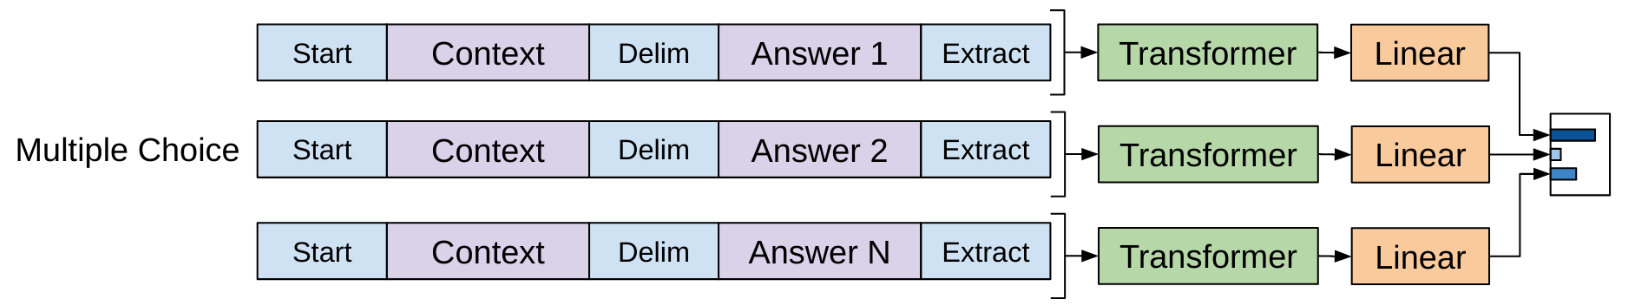
\includegraphics[width=0.8\textwidth]{multiple-choice.png}
    \caption{How multiple choice tasks are inlined to work with fine-tuning of \acrshort{acr:gpt} models \citep[4]{radfordImprovingLanguageUnderstanding2018}}
    \label{fig:multiple-choice}
\end{figure}

OpenAI's \acrshort{acr:api} currently features three flagship models, which are all proprietary|: the \acrshort{acr:gpt}-3.5 Turbo model, which is fast and inexpensive; the \acrshort{acr:gpt}-4 Turbo model, which as of \today~is described by OpenAI as their \enquote{previous high-intelligence model}; and lastly, \acrshort{acr:gpt}-4o, their \enquote{fastest and most affordable flagship model}.\footnote{\url{https://openai.com/api/}} The latter model has unique multi-modal abilities and can reason across audio, vision, and text in real time, according to OpenAI.\footnote{\url{https://openai.com/index/hello-gpt-4o/}}

\subsubsection{The Gemini Family}
\label{subsubsec:gemini}

The suite of models known as Gemini is Google's latest response OpenAI's \acrshort{acr:gpt} models. The Gemini 1.0 suite \citep{geminiteamGeminiFamilyHighly2024}, which is the first suite of Gemini models, includes three different models: Ultra, Pro, and Nano. These are listed in descending order in terms of size (number of model parameters). The models of the Gemini 1.0 suite are multi-modal, supporting text, image, audio, and video. Gemini 1.0 Ultra displayed new state-of-the-art performance on most major benchmarks, but performed significantly worse on the HellaSwag benchmark (which measures a model's common-sense understanding) compared to the latest \acrshort{acr:gpt}-4 model at the time. The models scored 87.8\% and 95.3\%, respectively. Supporting a context length up to 1M tokens, Gemini 1.0 Ultra surpassed Claude 2.1's context window of 200k (see the next paragraph for more on the Claude models) with a wide margin, and with the release of Gemini 1.5 Pro came also the possibility of utilizing a context window of up to 10M tokens, though in production this number is currently limited to 1M \citep{geminiteamGeminiUnlockingMultimodal2024, pichaiOurNextgenerationModel2024}. Furthermore, Gemini 1.5 Pro outperforms Gemini 1.0 Ultra in some capabilities despite using significantly less training compute \citep[31]{geminiteamGeminiUnlockingMultimodal2024}.

\subsubsection{The Claude Family}
\label{subsubsec:claude}

Developed at Anthropic, Claude is the third major suite of proprietary \acrshort{acr:llm}. Anthropic is one of the actors in the \acrshort{acr:llm} market that has helped push in the direction of long-context \acrshortpl{acr:llm}, with their Claude 2 model (released in November 2023) being the first to support up to 200k tokens \citep[9]{anthropicModelCardEvaluations2023}. Latest in line is Claude 3, a family of language models that ---- much like the Gemini family --- features three models of different sizes: Opus, Sonnet, and Haiku. Again, these are listed in descending order in terms of number of parameters. Opus offers the most advanced capabilities, and outperforms \acrshort{acr:gpt}-4 and Gemini 1.0 Ultra on most benchmarks \citep[6]{anthropicClaudeModelFamily2024}. Haiku is Anthropic's fast and economical option, while Sonnet serves as a balance between Opus' complexity and Haiku's speed.

\subsubsection{Open-Source Alternatives}
\label{subsubsec:open-source-llms}

As mentioned, OpenAI's \acrshort{acr:gpt} models, Google's Gemini models, and Anthropic's Claude models are all proprietary. This prevents developers from downloading these models and making improvements and customizations to them through fine-tuning. This, and several other reasons, have led to the emergence of a number of \textit{open-source} \acrshortpl{acr:llm}.

The \textbf{Llama} family of \acrshortpl{acr:llm}, developed at Meta AI, is perhaps the most famous open-source option to the proprietary \acrshortpl{acr:llm}. At the time of writing, the last in line is the \acrshort{acr:llama} 3 model \citep{metaaiIntroducingMetaLlama2024}, which comes in two sizes: 8B and 70B parameters. Both models display state-of-the-art performance on most major benchmarks compared to comparable open-source alternatives, and the 70B model even surpasses proprietary models like Gemini 1.5 Pro and Claude 3 Sonnet on certain benchmarks.

\textbf{Mistral AI} is one of the most prominent actors in the world of open-source \acrshortpl{acr:llm}. Their debut model, Mistral 7B, outperformed \acrshort{acr:llama} 2 13B (which was the best open-source \acrshort{acr:llm} at the time) across all the benchmarks they evaluated \citep{jiangMistral7B2023}. Mistral AI has also gained fame for their \gls{acr:smoe} architecture, which was introduced with the Mixtral 8x7B model \citep{jiangMixtralExperts2024}. It shares the same architecture as Mistral 7B, except that each layer of the model is composed of 8 feed-forward blocks. Using a router at each layer, Mixtral 8x7B is able to use only 13B out of a total of 47B parameters during inference, keeping cost and latency low.

Along with their Gemini models, Google released a family of open-source models called \textbf{Gemma}, which are based on the same research conducted for their Gemini models \citep{gemmateamGemmaOpenModels2024}. Gemma comes in two sizes: 2B and 7B parameters. At its release, the Gemma 7B surpassed \acrshort{acr:llama} 2 13B and Mistral 7B \acrshortpl{acr:llm} in 11 out of 18 benchmarks. Note, however, that \acrshort{acr:llama} 3 8B has improved upon its predecessor and now also performs better than Gemma 7B, overall.


\subsection{Prompt Engineering}
\label{subsec:prompt-engineering}

Prompt engineering refers to the process of constructing a query that will be used as input to an \acrshort{acr:llm}. In a chat-based context like that of ChatGPT, the prompt generally consists of a series of messages. These messages can hold one of three different roles\footnote{\url{https://platform.openai.com/docs/guides/text-generation/chat-completions-api}}, each listed below:

\begin{itemize}
    \item \textbf{System}: Generally used to set the behaviour of the \acrshort{acr:llm} assistant, giving the assistant a specific personality or information on how to answer the user.
    \item \textbf{User}: A message from the human user that the assistant should respond to.
    \item \textbf{Assistant}: A message generated by the \acrshort{acr:ai}/\acrshort{acr:llm}.
\end{itemize}

\cite{whitePromptPatternCatalog2023a} stress the importance of prompt engineering to efficiently converse with \glspl{acr:llm}. They provide a catalogue of prompt patterns that aim to help enforce certain qualities of the output generated by the \gls{acr:llm}. These patterns are organized into six distinct categories \citep[4]{whitePromptPatternCatalog2023a}:

\begin{itemize}
    \item \textbf{Input Semantics}: Clarifying what information is fed into the \acrshort{acr:llm} and how this input should be used to generate responses.
    \item \textbf{Output Customization}: Strategies to guide how the \acrshort{acr:llm} should format and structure its responses.
    \item \textbf{Error Identification}: Methods to identifying and resolving errors in the outputs produced by the \acrshort{acr:llm}.
    \item \textbf{Prompt Improvement}: Techniques to improve the quality of both the input provided to the \acrshort{acr:llm} and the output it generates.
    \item \textbf{Interaction}: Strategies for enhancing interactions between the user and the \acrshort{acr:llm}.
    \item \textbf{Context Control}: Controlling the contextual domain within which the \acrshort{acr:llm} operates.
\end{itemize}

Patterns that turned out useful to GeoGPT --- the main contribution of this thesis --- include the \textit{Template} pattern (Output Customization), the \textit{Reflection} pattern (Error Identification), and the \textit{Infinite Generation} pattern (Interaction Strategy). The \textit{Template} pattern allows the user or the system to define a template for the \acrshort{acr:llm} to fill out. This is closely related to function calling, which is discussed in \autoref{subsec:function-calling}. Also related to function calling is the \textit{Reflection} pattern, which allows the \acrshort{acr:llm} to inspect its own output in order to identify and correct errors. The \textit{Infinite Generation} pattern lets the \acrshort{acr:llm} generate output indefinitely without requiring the user to re-enter the conversation after each generated message. This pattern is important when developing agentic behaviours for the \acrshort{acr:llm}.


\subsection[Function Calling LLMs]{Function Calling \acrshortpl{acr:llm}}
\label{subsec:function-calling}

\textit{Function calling} --- also known as \textit{tool calling} --- was first introduced by OpenAI in April 2023 \citep{eletiFunctionCallingOther2023}. Function calling allows developers to provide function definitions to an \gls{acr:llm} and have the \gls{acr:llm} output a \acrshort{acr:json} object containing the name of one or more of the functions provided, as well as suitable parameters to these functions. \autoref{code:tool-definition-example} shows a description of a function that performs a mathematical division. Function calling \acrshortpl{acr:llm} are able to detect when a certain function should be called based on the name, description, and input parameters specified in such \acrshort{acr:json} objects. Function calling makes it possible to give an \gls{acr:llm} \textit{hooks} into the real world, and provides a more reliable way for developers to integrate \glspl{acr:llm} into applications.

\begin{lstlisting}[
    language=json,
    caption=Example of a tool definition,
    label=code:tool-definition-example
]
{
  "type": "function",
  "function": {
    "name": "divide",
    "description": "Performs a mathematical division.",
    "parameters": {
      "type": "object",
      "properties": {
        "dividend": {
          "description": "The number to be divided (numerator).",
          "type": "number"
        },
        "divisor": {
          "description": "The number by which the dividend is divided (denominator).",
          "type": "number"
        }
      },
      "required": ["dividend", "divisor"]
    }
  }
}
\end{lstlisting}

Function calling can be used to provide correct and up-to-date information that would otherwise require extensive training and fine-tuning. Having the \gls{acr:llm} use function calling for information retrieval also make them more transparent, making it possible to trace a claim back to its source, something that is normally hard to do with \glspl{acr:llm}. Another use case is code execution. Take this rather simple function signature:

$$
    \texttt{execute\_python\_code(code: string) -> string}
$$

Such a function could take some Python code as a string parameter and return the standard output that results from executing that code. This is the principle behind what was previously known as ChatGPT's \enquote{Code Interpreter} mode, where ChatGPT serves as a code executing agent that can generate, execute, and self-correct its own code. Similar functions could be constructed for \acrshort{acr:sql}, making it possible for \glspl{acr:llm} to work against relational databases. Furthermore, as \cite{eletiFunctionCallingOther2023} describes, function calling can also be used to extract structured data from text.

An initiative amongst researchers at Berkeley \citep{yanfanjiaBerkeleyFunctionCalling2024} lead to the creation of a benchmark that aims to evaluate the \acrshort{acr:llm}'s ability to call functions and tools. The benchmark, named \gls{acr:bfcl}, includes four different test scenarios: \textit{single function accuracy}, where the \acrshort{acr:llm} is provided with a single function definition; \textit{multiple function accuracy}, where 2 to 4 functions are passed and the model must select the appropriate function; \textit{parallel function}, where the model needs to determine how many functions should be called; and \textit{parallel multiple function}, a combination of parallel function and multiple function. Some models support different levels of function calling natively, while others have to be carefully prompted to help accommodate function calling abilities. At the time of writing (\today), a prompted version of \acrshort{acr:gpt}-4-0125-Preview tops the leaderboard.\footnote{\url{https://gorilla.cs.berkeley.edu/leaderboard.html}}

\section{LangChain}
\label{sec:langchain}

LangChain \citep{langchainaiLangchainaiLangchain2022} is an open-source project that provides tooling which simplifies the way developers interface with \glspl{acr:llm}. As the name suggests, LangChain revolves around \textit{chains}. Chains are \glspl{acr:dag}, which can be constructed from so-called \textit{runnables}. The \enquote{Runnable} protocol is a standard interface, which makes enforces chains to implement \texttt{stream}, \texttt{invoke}, and \texttt{batch} methods, as well as their asynchronous counterparts. LangChain is supported by a large community of developers, and has components that simplify interaction with \acrshortpl{acr:llm}, like prompt templates, output parsers, toolkits for function calling purposes, and off-the-shelf agents.

Common use cases for LangChain are:

\begin{itemize}
    \item Building chatbots for question answering that use semantic retrieval from document store
    \item Creating agents with access to external tools be leveraging function calling (see \autoref{subsec:function-calling})
    \item Creating code executing agents for Python, \acrshort{acr:sql}, or other programming languages
\end{itemize}

In January 2024, LangChain AI rolled out a framework called LangGraph, which is built on top of the LangChain ecosystem. While \textit{chains} are well-suited for \gls{acr:dag} workflows, they are not easily adapted to cyclic graphs. LangGraph, however, is specifically designed to simplify development of cyclic graphs for \acrshort{acr:llm} applications, which are commonly used to create agent-like behaviours \citep{langchainaiLangchainaiLanggraph2024}. A LangGraph \textit{graph} is a set of nodes that pass around and modify a state dictionary. The nodes are connected by edges that define what node can succeed another node. Edges can be conditional, meaning the state produced from one node decides which edge is followed. This allows for complex logic and simplifies implementation of advanced agent patterns, some of which are discussed in \autoref{subsec:agent-patterns}.


\section{Geospatial Databases and Data Catalogues}
\label{sec:geo-dbs-and-data-catalogues}

This section will discuss the geospatial technologies that were used or considered for use in this master's thesis.

\subsection{PostGIS}
\label{subsec:postgis}

PostGIS \citep{PostGIS2001} is an open-source extension for the PostgreSQL \acrshort{acr:dbms}. The PostGIS extension adds support for storing, indexing, and querying geospatial data. Data can be stored in both two and three dimensions, and they can have types like points, lines, polygons. Geospatial types can be stored along with a spatial index which can significantly reduce search time for their geometries. GiST (Generalized Search Tree)\footnote{\url{https://en.wikipedia.org/wiki/GiST}} is commonly used in PostgreSQL/PostGIS to take advantage of various tree-based search algorithms that are developed to retrieve spatial features quickly.

PostGIS also comes with a plethora of spatial database functions that are used to analyse and process geospatial data. These function's names are prefixed with \texttt{ST\_} (short for \enquote{spatio-temporal}), and some examples are \texttt{ST\_DWITHIN}, \texttt{ST\_BUFFER}, and \texttt{ST\_TRANSFORM}. \autoref{code:postgis-example} shows a typical query for retrieving building outlines within a bounding box.

\begin{lstlisting}[
    language=SQL,
    caption=PostGIS example code for retrieving building outlines within a specified bounding box,
    label=code:postgis-example
]
SELECT * 
FROM osm_buildings_polygons 
WHERE type = 'house' 
  AND ST_Intersects(geom, ST_MakeEnvelope(min_lon, min_lat, max_lon, max_lat, 4326));
\end{lstlisting}

\subsection[OGC API Features]{\acrshort{acr:ogc} \acrshort{acr:api} Features}
\label{subsec:ogc-api-features}

\acrshort{acr:ogc} \acrshort{acr:api} Features is an \acrshort{acr:api} specification that defines modular \acrshort{acr:api} building blocks for interacting with features, which are real-world objects \citep{opengeospatialconsortiumOGCAPIFeatures2022}. This includes blocks for creating, modifying, and querying features on the Web. A typical implementation of \acrshort{acr:ogc} \acrshort{acr:api} Features implements these building blocks for \acrshort{acr:html}, GeoJSON, and \acrshort{acr:gml}. These are called \textit{requirement classes}, though none of them are strictly required. The \acrshort{acr:html} requirement class gives the user of the \acrshort{acr:api} a visualization of the features, whereas the GeoJSON and \acrshort{acr:gml} requirements classes are typically meant for use in other applications.

\begin{figure}[h]
    \centering
    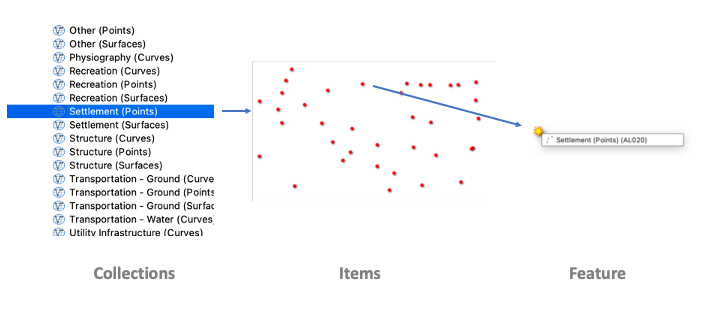
\includegraphics[width=\textwidth]{ogc_api_features.png}
    \caption{Collections, items, and features in \acrshort{acr:ogc} \acrshort{acr:api} Features specification. Retrieved from \url{https://features.developer.ogc.org/} on April 29, 2024.}
    \label{fig:oaf-collections-items-features}
\end{figure}

The development of the Features standard is divided into several parts that are meant to build on top of one another. Here are the five parts that are listed on \acrshort{acr:ogc}'s websites:\footnote{\url{https://ogcapi.ogc.org/features/}}

\begin{itemize}
    \item Features - Part 1: Core\footnote{\url{https://docs.opengeospatial.org/is/17-069r4/17-069r4.html}}
    \item Features - Part 2: Coordinate Reference Systems by Reference \footnote{\url{https://docs.ogc.org/is/18-058r1/18-058r1.html}}
    \item Features - Part 3: Filtering\footnote{\url{https://docs.ogc.org/DRAFTS/19-079r1.html}}
    \item Features - Part 4: Create, Replace, Update and Delete\footnote{\url{https://docs.ogc.org/DRAFTS/20-002.html}}
    \item Features - Part 5: Schemas\footnote{\url{https://docs.ogc.org/DRAFTS/23-058r1.html}}
\end{itemize}

Part 1 specifies core capabilities that are described in the first paragraph of this section, while parts 2-4 spcify additional capabilities. Part 2 allows for retrieval of features in \glspl{acr:crs} different to the default WGS 84 reference system. Part 3 enables filtering of features using \gls{acr:cql}. \gls{acr:cql} is a language similar to \acrshort{acr:sql}. This allows for filtering of collections, so that users of the \acrshort{acr:api} can retrieve subsets of a given collection. Below are two examples of \gls{acr:cql} queries:

\begin{lstlisting}[
    language=SQL,
    caption=\acrshort{acr:cql} examples,
    label=cql-examples
]
\\ Example 1
county in ('Akershus', 'Buskerud', 'Ostfold')

\\ Example 2
DWITHIN(the\_geom, Point(63.4265, 10.3960), 1, kilometers)
\end{lstlisting}

Part 4 defines how an \acrshort{acr:api} that implements the specification should handle addition, replacement, modification, and removal of a collection's features. Part 5 describes how features can be described by a logical schema and how these schemas are published. In addition to parts 1 through 5, several other \textit{proposed} extensions have emerged, such as the \textit{Search} extension, which would allow for multi-collection queries, or the \textit{Geometry Simplification} extension which proposes the use of simplification algorithms for retrieving simplified versions of a collection.\footnote{\url{https://github.com/opengeospatial/ogcapi-features/tree/master/proposals}}


\subsection[SpatioTemporal Asset Catalogs]{\acrlong{acr:stac}}
\label{subsec:stac}

The \gls{acr:stac} specification\footnote{\url{https://stacspec.org/en}} is closely related to \acrshort{acr:ogc} \acrshort{acr:api} Features, and Chris Holmes, former board member of \acrlong{acr:ogc}, stated in a blog post that \enquote{\acrshort{acr:stac} \acrshort{acr:api} implements and extends the \acrshort{acr:ogc} \acrshort{acr:api} — Features standard, and our shared goal is for \acrshort{acr:stac} \acrshort{acr:api} to become a full \acrshort{acr:ogc} standard} \citep{holmesSpatioTemporalAssetCatalogs2021a}. The main difference between \acrshort{acr:ogc} \acrshort{acr:api} Features and \acrshort{acr:stac} is the latter's requirement that all items/features should have a temporal component, thus making it \textit{spatio-temporal}.


\section{Related Work}
\label{sec:related-work}

The related work is divided into two main parts: \autoref{subsec:llm-gis}, which presents research investigating potential use cases of \acrshortpl{acr:llm} in the field of geospatial information technology; and \autoref{subsec:agent-patterns}, which presents examples of three different types of patterns commonly used in \acrshort{acr:llm}-based agents.

\subsection[Using LLMs for Geospatial Purposes]{Using \acrshortpl{acr:llm} for Geospatial Purposes}
\label{subsec:llm-gis}

\cite{robertsGPT4GEOHowLanguage2023} investigated the extent of GPT-4's geospatial awareness through a set of case studies with increasing difficulty, starting with general factual tasks and finishing with complex questions such as generating country outlines and travel networks. The authors found that \acrshort{acr:gpt}-4 is \enquote{skillful at solving a variety of application-centric tasks}, almost having the ability to \enquote{see}, despite being a language model and therefore only able to interface with the world through sequenced, textual input (note that multi-modal models were not particularly widespread when they wrote their paper). Examples include its ability to serve as a travel assistant in providing itinerary suggestions for a trip when provided with requirements, and its ability to provide generally correct start and end locations of bird migration paths. While it quickly became obvious that a lot of geospatial context have been embedded within the model during the vast pre-training, the question of whether this is memorization or reasoning is a central one. The authors suggest that the variability of tasks in their experiments deems it unlikely that it is all memorization, but they say that some things appear to be memorized.

\cite{mooneyUnderstandingGeospatialSkills2023} examined the performance of ChatGPT in a \acrfull{acr:gis} exam, aiming to assess its ability to grasp various geospatial concepts, highlighting its capabilities and limitations. Experiments were conducted on GPT-3.5 and GPT-4, which delivered performances equivalent to grades of D and B+, respectively. Additional experiments were conducted for more specialized areas of \acrshort{acr:gis}, including True/False questions about spatial analysis, and simple tasks in applied \acrshort{acr:gis} workflows. Experiments on the latter showed that GPT-4 was able to correctly answer a relatively complex \acrshort{acr:gis} task involving seven different datasets, requiring seven steps in order to obtain a perfect score. Generally, GPT-4 outperformed GPT-3.5 in all tasks. While clearly powerful, the authors highlight a range of challenges, among which the multi-modal nature of \acrshort{acr:gis}.

\cite{liAutonomousGISNextgeneration2023} state that \enquote{autonomous \acrshort{acr:gis} will need to achieve five autonomous goals: self-generating, self-organizing, self-verifying, self-executing, and self-growing.}. They provide a \enquote{divide-and-conquer}-based method to address some of these goals. Furthermore, they propose a simple trial-and-error approach to address the self-verifying goal. They also highlight the need for a memory system in a mature \acrshort{acr:llm}-based \acrshort{acr:gis} system, referring to the use of vector databases in autonomous agents made with frameworks like AutoGPT \citep{richardAutoGPTHeartOpensource2023}. Even with its shortages, the solution that \cite{liAutonomousGISNextgeneration2023} provide, called \acrshort{acr:llm}-Geo, is able to produce good solutions in various case studies by providing executable assemblies in a Python environment when provided with URLs to relevant data sets, along with a user-specified query.

\cite{zhangGeoGPTUnderstandingProcessing2023} use the LangChain framework in order to combine different GIS tools in a sequence to solve various sub-goals, focusing on using the semantic understanding and reasoning abilities of \acrshortpl{acr:llm} to call externally defined tools, employing the \acrshort{acr:llm} as an agent or controller. The authors take great inspiration from the AutoGPT framework \citep{richardAutoGPTHeartOpensource2023}. The externally defined tools are described by their names and descriptions. These descriptions contain information about the input parameters and output types of the tools/functions. Tools are defined for geospatial data collection, data processing and analysis, and data visualization. The effectiveness of the system is showcased through case studies.


\subsection{Agent Patterns}
\label{subsec:agent-patterns}

\acrshort{acr:llm}-based agents can be implemented in many different ways, and researchers have developed a plethora of \textit{agent patterns} that seek to improve upon areas where \acrshortpl{acr:llm} tend to be less effective.This section will shortly explain three different types of patterns that were considered during the development of GeoGPT.

The \textbf{multi-agent} pattern takes inspiration from human collaboration in that it is made up from multiple specialized agents that work together to achieve some objective. MetaGPT \citep{hongMetaGPTMetaProgramming2023} is a \acrshort{acr:llm}-based multi-agent system consisting of agents with human-level domain expertise. Using an assembly line paradigm, where the overall goal is divided into subtasks, \citeauthor{hongMetaGPTMetaProgramming2023} showed that MetaGPT could generate more coherent solutions compared to the previous state-of-the-art multi-agent systems. At the time of release, MetaGPT set a new state-of-the-art performance on the HumanEval and \acrshort{acr:mbpp} benchmarks \citep[7]{hongMetaGPTMetaProgramming2023}, demonstrating the potential of the multi-agent pattern. AutoGen \citep{wuAutoGenEnablingNextGen2023a} and crewAI \citep{mouraJoaomdmouraCrewAI2024} are other examples of frameworks geared towards the multi-agent pattern.

Patterns that employ \textbf{self-reflection} are commonly used with autonomous \acrshort{acr:llm}-based agents. \textit{Reflextion} \citep{shinnReflexionLanguageAgents2023} is a framework that reinforces agents through linguistic feedback, essentially allowing the agent to reflect upon the outcomes of its actions. The framework utilizes three distinct models: an \textit{Actor} model responsible for generating text and actions; an \textit{Evaluator} model which assessses the quality of the outputs from the Actor; and a \textit{Self-Reflection} model that generates reinforcement cues for the Actor based on the output and quality assessment of the other two models. Together, these three models form a loop that will run until the Evaluator deems the output from the Actor as correct.

\textbf{Step-by-step reasoning} is another pattern that has proved to be efficient in helping \acrshortpl{acr:llm} produce correct responses. \cite{weiChainofThoughtPromptingElicits2023a} demonstrated that so-called \textit{chain-of-thought prompting} can be used for enhancing reasoning in \acrshortpl{acr:llm} by providing it with examples of how to reason for tasks \textit{similar} to that which it is trying to solve. By helping the \acrshort{acr:llm} with decomposing multi-step problems into intermediate steps, \citeauthor{weiChainofThoughtPromptingElicits2023a} managed to achieve state-of-the-art accuracy on the GSM8K benchmark of math word problems.


\glsresetall
